\documentclass[a4paper]{article}

\title{Protein HMM}
\author{Danilo Horta}
\date{August 2019}

\usepackage{natbib}
\usepackage{graphicx}
\usepackage{amsmath}
\usepackage{amsthm}
\usepackage{amssymb}
\usepackage[margin=0.5in]{geometry}
\usepackage{rotating}
\usepackage{subcaption}
\usepackage[T1]{fontenc}
\usepackage{mathtools}

\theoremstyle{definition}
\newtheorem{example}{Example}[section]

\theoremstyle{definition}
\newtheorem{definition}{Definition}[section]

\theoremstyle{definition}
\newtheorem{corollary}{Corollary}[section]

\newcommand{\prob}[1]{p (#1)}
\newcommand{\cprob}[2]{p\left(#1\;\middle|\; #2\right)}
\newcommand{\eps}{\epsilon}
\newcommand{\s}{\texttt{\char`_}}
\newcommand{\gv}{\;|\;}
\newcommand*{\field}[1]{\mathbb{#1}}%
\newcommand*{\set}[1]{\mathcal{#1}}%
\newcommand*{\arr}[1]{\mathbf{#1}}%
\newcommand{\eqdef}{\coloneqq}

\begin{document}

\maketitle

\abstract{Lorem ipsum dolor sit amet, consectetur adipiscing elit. Phasellus eu felis
    felis. Sed turpis nibh, laoreet a aliquam sit amet, condimentum at leo. Nunc vitae
    ipsum quis magna mollis lacinia nec a est. Donec aliquam aliquet tortor vel rhoncus.
    Duis mi erat, vehicula a sem eget, tincidunt malesuada nulla. Aliquam pellentesque
  posuere nibh nec elementum. Quisque eu accumsan justo, ac viverra nibh.}

\section{Model}

\begin{definition}\label{def:mp}
  A Markov process is a stochastic process $Q_1, \dots$ for which
  \begin{equation*}
    p(Q_t=q_t \gv Q_1=q_1, Q_2=q_2, \dots, Q_{t-1}=q_{t-1}) = p(Q_t=q_t \gv Q_{t-1}=q_{t-1}).
  \end{equation*}
  The possible values of $Q_t$ form a finite set $\set{Q}$ called the state space.
\end{definition}

\begin{definition}\label{def:hmm}
  Let $\set{A}$ be a non-empty finite set of symbols. Let $Q_1, Q_2, \dots$ be a Markov process and
  let $S_1, S_2, \dots$ be a stochastic process for which
  \begin{equation*}
    p(S_t\in\set{A} \gv Q_1=q_1, Q_2=q_2, \dots, Q_t=q_t) = p(S_t\in\set{A} \gv Q_t=q_t).
  \end{equation*}
  The pair $(Q_t, S_t)$ is a hidden Markov model (HMM) with alphabet $\set{A}$.
\end{definition}

Let $\arr{z}=z_1 .. z_L$ be a sequence emitted by an HMM.\@
The marginal likelihood of $\arr{z}$ is defined by
\begin{equation}\label{eq:hml}
  \mathrm{ML}(\arr{z}) \eqdef p(S_1=z_1, S_2=z_2, \dots, S_L=z_L).
\end{equation}

The standard HMM definition is often extended to include states that do not emit symbols. Those
states are referred to as silent states and are useful to describe a missing alignment position, for
example. This section goes a step further by defining a more general hidden Markov model that
accounts for states that instead emit sequence of symbols of variable length, including zero-length
sequences.

\begin{definition}
  Let $\set{A}$ be a non-empty finite set of symbols, $k\in\field{N}_0$, and define
  $\set{B}=\bigcup_{i=0}^k\set{A}^i$.
  Let $Q_1, Q_2, \dots$ be a Markov process and let $S_1, S_2, \dots$ be a stochastic process for
  which
  \begin{equation*}
    p(S_t\in\set{B} \gv Q_1=q_1, Q_2=q_2, \dots, Q_t=q_t)
    = p(S_t\in\set{B} \gv Q_t=q_t).
  \end{equation*}
  The pair $(Q_t, S_t)$ is an invisible Markov model (IMM) with alphabet $\set{A}$ and
  limit $k$.
\end{definition}

Let $\arr{z}=z_1 .. z_L$ be a sequence emitted by an IMM.\@
The marginal likelihood of $\arr{s}$ cannot be written as in Eq.~\eqref{eq:hml} since
we've lost the the order association between symbols and states.
Instead, the marginal likelihood is given by
\begin{equation}\label{eq:ml}
  \mathrm{ML}(\arr{z}) \eqdef \sum_{t=1}^{\infty} p(S_{1..t}=\arr{z}, S_{t+1}\neq \emptyset),
\end{equation}
where $S_{1..t}$ denotes the concatenation of the random variables $S_1$, $S_2$,
$\dots$, and $S_t$.\footnote{For example, let $a$ be a symbol. We have
$p(S_{1..2}=a) = p(S_1=a, S_2=\emptyset) + p(S_1=\emptyset, S_2=a)$.}

\subsection{Viterbi}

Let us consider first the Viterbi method applied to HMMs.
Let
\begin{equation*}
  \viterbi(q_t) \eqdef \umax{q_{1..t-1}} \{ p(S_{1..t}=z_{1..t}, Q_{1..t}=q_{1..t}) \}
\end{equation*}
be the so-called Viterbi score.
It is the maximum probability among all state paths that ends in $q_t$ and generates
the sequence $z_{1..t}$.

Viterbi score can also be defined in a recursive fashion as follows:
\begin{equation*}
\begin{split}
  \viterbi(q_t)
  &= p(S_t=z_t \gv Q_t=q_t) \umax{q_{1..t-1}}
    \{ p(Q_t=q_t \gv Q_{t-1}=q_{t-1}) p(S_{1..t-1}=z_{1..t-1}, Q_{1..t-1}=q_{1..t-1}) \} \\
  &= p(S_t=z_t \gv Q_t=q_t) \umax{q_{t-1}}
    \{ p(Q_t=q_t \gv Q_{t-1}=q_{t-1})
    \umax{q_{1..t-2}} \{ p(S_{1..t}=z_{1..t-1}, Q_{1..t}=q_{1..t-1}) \} \} \\
  &= p(S_t=z_t \gv Q_t=q_t) \umax{q_{t-1}} \{ p(Q_t=q_t \gv Q_{t-1}=q_{t-1})
    \viterbi(q_{t-1}) \}
\end{split}
\end{equation*}

Let $i \leq L$ indicate the prefix $z_{1:i}$.
We define
\begin{align*}
  \mathcal{V}_{q_t,f_t}(i) =
  \max_{q_{t-1}, f_{t-1}}
  \big\{
    \mathcal{V}_{q_{t-1},f_{t-1}}(i-f_t) p(V_t=z_{i-f_t+1:i} \gv Q_t=q_t) p(Q_t=q_t \gv
    Q_{t-1}=q_{t-1})
  \big\},
\end{align*}
for $0 < i - f_t$,
and
\begin{align*}
  \mathcal{V}_{q_t,f_t}(i) =
  \max
  \Big\{
    &\max_{q_{t-1}}
    \big\{
      \mathcal{V}_{q_{t-1}}(0) p(V_t=z_{1:i} \gv Q_t=q_t) p(Q_t=q_t \gv
      Q_{t-1}=q_{t-1})
    \big\},\\
    &p(V_t=z_{1:i} \gv Q_t=q_t) p(Q_t=q_t)
  \Big\},
\end{align*}
for $0 = i - f_t$.

The maximal probability over all state paths $q_1, q_2, \dots$ and emission lengths $f_1, f_2,
\dots$ is given by
\begin{align*}
  \max_{q_t, f_t}\mathcal{V}_{q_t,f_t}(L).
\end{align*}

\subsection{Not sure}

Let $q_{1..t}$ be a sequence of states (also known as state path).
The likelihood of sequence $\arr{z}$ for state path $q_{1..t}$ is given by
\begin{align*}
  \mathrm{L}(\arr{z}, q_{1..t}) = p(V_{1..t}=\arr{z}, Q_{1..t}=q_{1..t}).
\end{align*}
Note that
\begin{align*}
  \mathrm{L}(\arr{z}, q_{1..t}) &= \sum_{l_t=0}^L p(V_{1..t}=\arr{z}, L_t=l_t,
  Q_{1..t}=q_{1..t})\\
  &= \sum_{l_t=0}^L p(V_{1..t-1}=z_{1..l_t}, V_t=z_{l_t+1..L}, Q_{1..t-1}=q_{1..t-1}, Q_t=q_t)\\
  &= \sum_{l_t=0}^L p(V_t=z_{l_t+1..L} \gv Q_t=q_t) p(Q_t=q_t \gv Q_{t-1}=q_{t-1})
  \mathrm{L}(z_{1..l_t}, q_{1..t-1})
\end{align*}

% Let
% \begin{align*}
%   \mathrm{L}(z_{1..l_t}, z_{l_t+1..l_t+f_t}, q_{1..t})
%   &= p(V_t=z_{l_t+1..l_t+f_t} \gv Q_t=q_t) p(Q_t=q_t \gv Q_{t-1}=q_{t-1})\\
%   &p(V_{1..t-1} = z_{1..l_t}, Q_{1..t-1}=q_{1..t-1}).
% \end{align*}
% Let
% \begin{align*}
%   g_t(z_{1..l_t}, z_{l_t+1..l_t+f_t}, q_t)
%   &= \max_{q_{t-1}, f_{t-1}}
%   \Big\{
%     p(V_t=z_{l_t+1..l_t+f_t} \gv Q_t=q_t) p(Q_t=q_t \gv Q_{t-1}=q_{t-1}) \\
%     &g_{t-1}(z_{1..l_{t-1}}, z_{l_{t-1}+1..l_{t-1}+f_{t-1}}, q_{t-1})
%   \Big\}.\\
%   g_1(\emptyset, z_{1..f_1}, q_1)
%   &= p(V_1=z_{1..f_1} \gv Q_1=q_1) p(Q_1=q_1)
% \end{align*}

\subsection{Discussion}

For computational reasons, it would be useful to have an upper bound on the summation of the
marginal likelihood.
We will define a type of IMM that has such a feature.

\begin{definition}
  A cycle is any probable sequence of states that starts and ends with the same state.
\end{definition}

\begin{definition}
  A quiet state is a state that has a non-zero probability of emitting an empty sequence.
\end{definition}

\begin{definition}
  A quiet cycle is any cycle having only quiet states.
\end{definition}

\begin{corollary}
  Let $M$ be the number of states of the IMM.\@ If it has no quiet cycles, any sequence of $M$ states
  will have emitted at least one symbol.
\end{corollary}

If IMM has no quiet cycles, there is always a $N \leq L\cdot M$ such that
\begin{equation*}
  \mathrm{ML}(\arr{z}) = \sum_{t=1}^{L\cdot M} p(V_{1..t}=\arr{z}, L_t<L).
\end{equation*}

\section{Frame}

Let $(Q_t, S_t)$ be a HMM with the amino acid alphabet $\set{A}$.
We want to replace it with a HMM that generates sequences of symbols from the alphabet
$\mathcal B = \{\mathrm A, \mathrm C, \mathrm G, \mathrm T\}$ of DNA bases and is able to account
for frame-shifting.
Let $\mathrm M_j$ be the so-called match state of an amino acid HMM and let $Q_t=\mathrm M_j$.
From the amino acid emission probabilities and any other relevant source of information
(codon usage bias, for instance), one can define the probability $\cprob{X_1=x_1, X_2=x_2, X_3=x_3}{Q_t=\mathrm M_j}$
of $\mathrm M_j$ emitting the codon $(x_1, x_2, x_3) \in \mathcal B^3$
--- one can also write $\cprob{X=x_1x_2x_3}{Q_t=\mathrm M_j}$, for short.
Since measurement errors occur and nature is not perfect, we will replace the
codon emission process by one that instead produces base sequences of different
lengths to account for base insertions and deletions (indels).

Node $\mathrm M_j$ in Fig.~\ref{fig:codon-hmm-tree} represents the modified match state.
The generated codon will go through four transitions, each one representing one of three possibilities: (i) delete a base; (ii) insert a base; or (iii) do nothing.
The deletion can happen in any of the three codon positions with equal probability.
If a deletion has already happened, the next deletion can happen in any of the remaining two positions with equal probability.
The insertion can happen between any two bases, before the first base or after the last base with equal probability.

The codon emitted at node $\mathrm M_j$ can go under $m\in\{0, 1, 2, 3, 4\}$ base indels during
the state transitions that end at some leaf-node state.
The probability of it undergoing $m$ indels is given by
\begin{align*}
    p(M=m) = \binom{4}{4-m} (1 - \eps)^{4-m} \eps^m,
\end{align*}
where coefficient $\binom{4}{m}$ counts the number of paths corresponding to $m$ base indels.
Fig.~\ref{fig:indel-dist} shows the base indel distributions over different values of $\eps$.
Let $F$ be a random variable representing the final sequence length generated by the model in
Fig.~\ref{fig:codon-hmm-tree}.
We have the probabilities
\begin{align*}
    p(F=1) = p(F=5) &= \eps^2(1-\eps)^2, \\
    p(F=2) = p(F=4) &= 2\eps^3(1-\eps) + 2\eps(1-\eps)^3,~\text{and} \\
    p(F=3)          &= \eps^4 + 4\eps^2(1-\eps)^2 + (1-\eps)^4
\end{align*}
illustrated in Fig.~\ref{fig:len-dist} over different values of $\eps$.

\begin{figure}[htbp]
\centering
\begin{subfigure}{.5\textwidth}
  \centering
  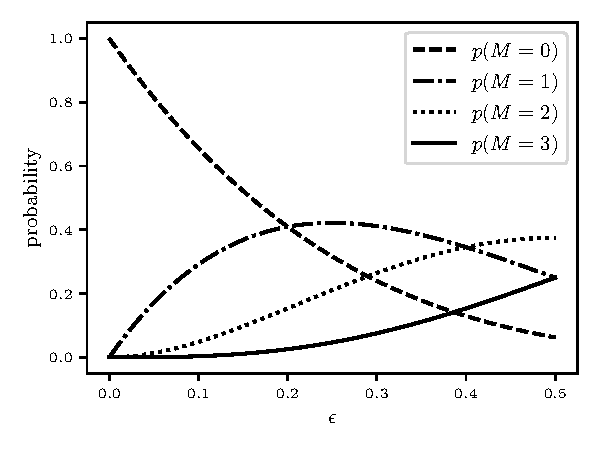
\includegraphics[width=.7\linewidth]{figure/indel-prob}
  \caption{Base indel distribution.}%
  \label{fig:indel-dist}
\end{subfigure}%
\begin{subfigure}{.5\textwidth}
  \centering
  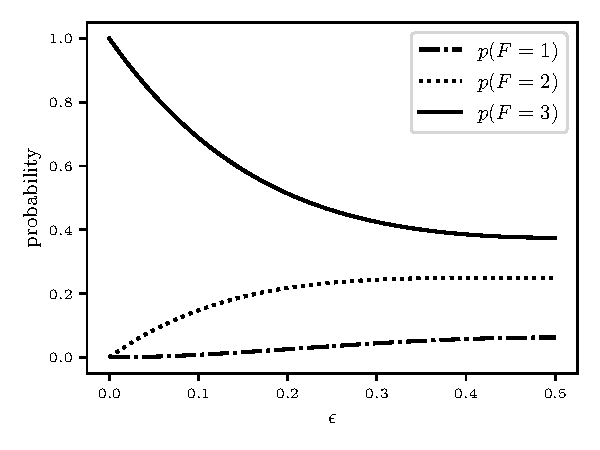
\includegraphics[width=.7\linewidth]{figure/seq-len-prob}
  \caption{Sequence length distribution.}%
  \label{fig:len-dist}
\end{subfigure}
\caption{
    Distribution of base indels and sequence length over the transition probability $\eps$.
    It is recommended to choose a value for $\eps$ that is smaller than $1/5$ such that
    $p(M=m)<p(M=m+1)$, as per Fig.~\ref{fig:indel-dist}.
}
\label{fig:dist}
\end{figure}

A sequence $\mathbf z=z_1 z_2\dots$ of finite but variable length will emerge at the end of the
process represented in Fig.~\ref{fig:codon-hmm-tree}.
Let $\mathcal Q_f$ be the set of hidden paths, starting with $Q_t=\mathrm M_j$ and ending at some leaf-node state,
that generate sequences of length $f$.
Let $Z^f=(Z^f_1, \dots, Z^f_f)$ be a $f$-tuple of random variables that generates such sequences of length $f$.
We have
\begin{align*}
    p(Z^f=z_1\dots z_f,F=f) &= \sum_{\mathbf q \in \mathcal Q_f}
    \cprob{Z^f=z_1\dots z_f}{Q_{t..t+4}=\mathbf q} p(Q_{t..t+4}=\mathbf q).
\end{align*}

\section{Final sequence distribution}

We will write $p(X=x_1x_2x_3) = p(X=x_1x_2x_3 \gv Q_t = \mathrm M_j)$ for brevity.
Underscore $\s$ denotes a summation over the corresponding random variables.
For example, $p(X=x_1\s\s)=\sum_{x_2,x_3}p(X=x_1x_2x_3)$.

\subsection{Sequences of length 1}

\begin{equation*}
  p(Z^1=z_1,F=1) = \eps^2(1-\eps)^2(p(X=z_1\s\s) + p(X=\s z_1\s) + p(X=\s\s z_1)) / 3
\end{equation*}

\subsection{Sequences of length 2}

\begin{equation*}
  \begin{split}
    p(Z^2=z_1z_2,F=2)
        &= 2\eps(1-\eps)^3(p(X=\s z_1z_2) + p(X=z_1\s z_2) + p(X=z_1z_2\s))/3\\
        &+ \eps^3(1-\eps)(p(X=z_1\s\s) + p(X=\s z_1\s) + p(X=\s\s z_1))p(z_2)/3\\
        &+ \eps^3(1-\eps)(p(X=z_2\s\s) + p(X=\s z_2\s) + p(X=\s\s z_2))p(z_1)/3
  \end{split}
\end{equation*}

\subsection{Sequences of length 3}

\begin{equation*}
  \begin{split}
    p(Z^3=z_1z_2z_3,F=3) &= (1-\eps)^4 p(X=z_1z_2z_3)\\
        &+ 4\eps^2(1-\eps)^2 (p(X=\s z_2 z_3) + p(X=z_2\s z_3) + p(X=z_2 z_3\s))p(z_1)/9\\
        &+ 4\eps^2(1-\eps)^2 (p(X=\s z_1 z_3) + p(X=z_1\s z_3) + p(X=z_1 z_3\s))p(z_2)/9\\
        &+ 4\eps^2(1-\eps)^2 (p(X=\s z_1 z_2) + p(X=z_1\s z_2) + p(X=z_1 z_2\s))p(z_3)/9\\
        &+ \eps^4 (p(X=z_3\s\s) + p(X=\s z_3\s) + p(X=\s\s z_3))p(z_1)p(z_2)/9\\
        &+ \eps^4 (p(X=z_2\s\s) + p(X=\s z_2\s) + p(X=\s\s z_2))p(z_1)p(z_3)/9\\
        &+ \eps^4 (p(X=z_1\s\s) + p(X=\s z_1\s) + p(X=\s\s z_1))p(z_2)p(z_3)/9
  \end{split}
\end{equation*}

\subsection{Sequences of length 4}

\begin{equation*}
  \begin{split}
    p(Z^4=z_1z_2z_3z_4,F=4) &= \eps(1-\eps)^3 (p(X=z_2z_3z_4)p(z_1)+p(X=z_1z_3z_4)p(z_2)\\
        &+p(X=z_1z_2z_4)p(z_3)+p(X=z_1z_2z_3)p(z_4))/2\\
        &+\eps^3(1-\eps)(\\
        &+ p(X=\s z_3z_4)p(z_1)p(z_2) + p(X=\s z_2z_4)p(z_1)p(z_3)\\
        &+ p(X=\s z_2z_3)p(z_1)p(z_4) + p(X=\s z_1z_4)p(z_2)p(z_3)\\
        &+ p(X=\s z_1z_3)p(z_2)p(z_4) + p(X=\s z_1z_2)p(z_3)p(z_4)\\
        &+ p(X=z_3\s z_4)p(z_1)p(z_2) + p(X=z_2\s z_4)p(z_1)p(z_3)\\
        &+ p(X=z_2\s z_3)p(z_1)p(z_4) + p(X=z_1\s z_4)p(z_2)p(z_3)\\
        &+ p(X=z_1\s z_3)p(z_2)p(z_4) + p(X=z_1\s z_2)p(z_3)p(z_4)\\
        &+ p(X=z_3z_4\s)p(z_1)p(z_2) + p(X=z_2z_4\s)p(z_1)p(z_3)\\
        &+ p(X=z_2z_3\s)p(z_1)p(z_4) + p(X=z_1z_4\s)p(z_2)p(z_3)\\
        &+ p(X=z_1z_3\s)p(z_2)p(z_4) + p(X=z_1z_2\s)p(z_3)p(z_4))/9
  \end{split}
\end{equation*}

\subsection{Sequences of length 5}

\begin{equation*}
  \begin{split}
    p(Z^5=z_1z_2z_3z_4z_5,F=5)
        &= \eps^2(1-\eps)^2(\\
        &+p(z_1)p(z_2)p(X=z_3z_4z_5)+p(z_1)p(z_3)p(X=z_2z_4z_5)\\
        &+p(z_1)p(z_4)p(X=z_2z_3z_5)+p(z_1)p(z_5)p(X=z_2z_3z_4)\\
        &+p(z_2)p(z_3)p(X=z_1z_4z_5)+p(z_2)p(z_4)p(X=z_1z_3z_5)\\
        &+p(z_2)p(z_5)p(X=z_1z_3z_4)+p(z_3)p(z_4)p(X=z_1z_2z_5)\\
        &+p(z_3)p(z_5)p(X=z_1z_2z_4)+p(z_4)p(z_5)p(X=z_1z_2z_3))/10
  \end{split}
\end{equation*}

\section{Model generalisation}

Fig.~\ref{fig:imm} illustrates a probabilistic graphical representation of the IMM.\@

\begin{figure}[htbp]
\centering
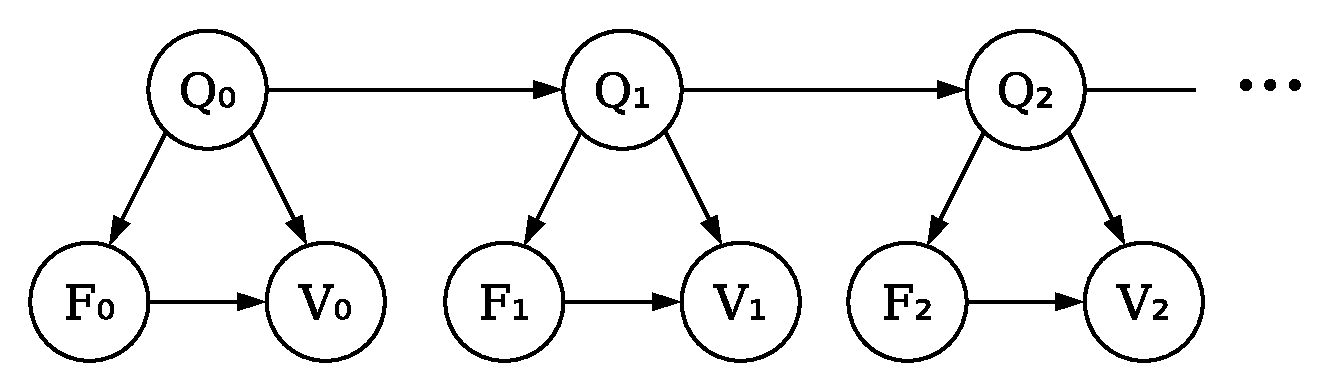
\includegraphics[width=.45\linewidth]{figure/imm}
\caption{Invisible Markov model.}%
\label{fig:imm}
\end{figure}

\newpage
\newpage

\begin{sidewaysfigure}[ht]
    \centering
    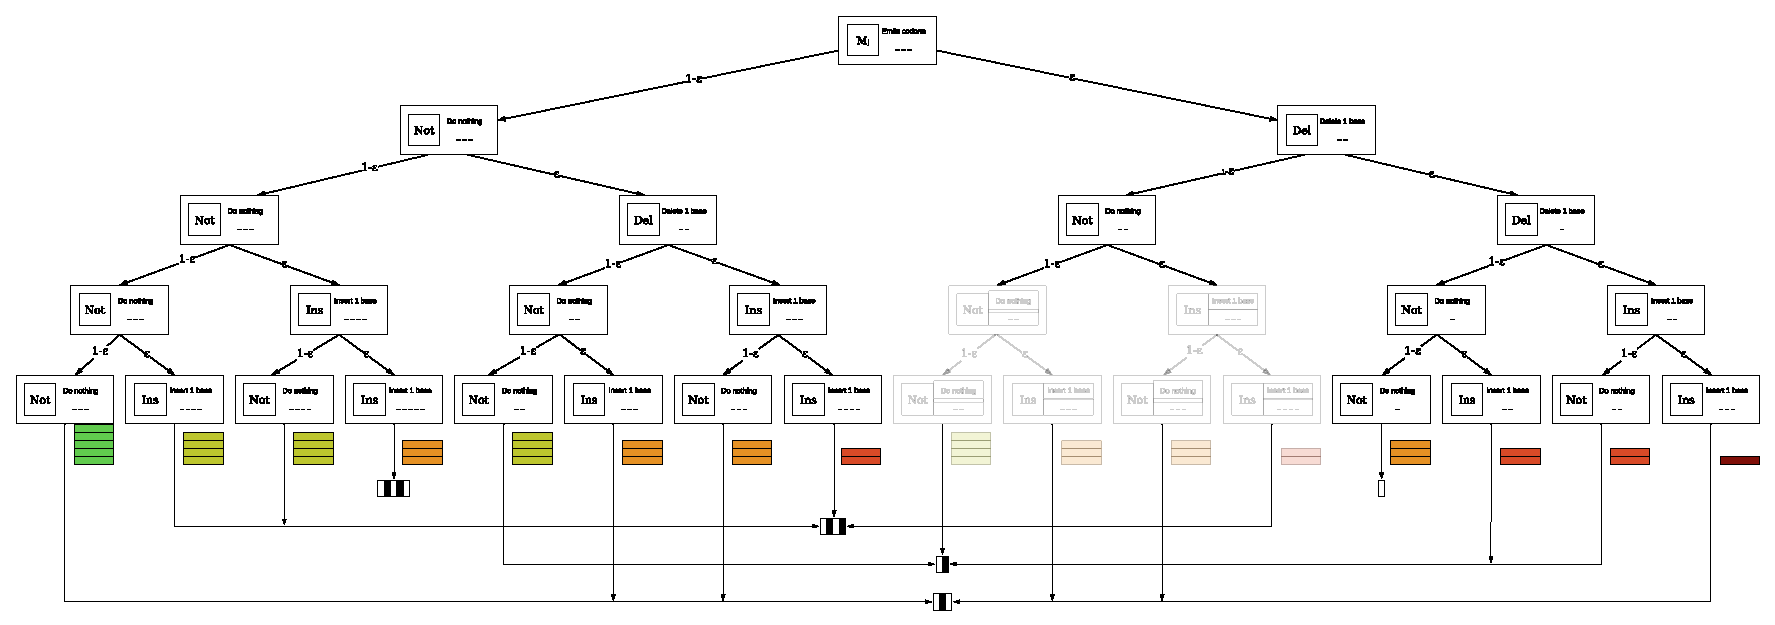
\includegraphics[scale=0.9]{figure/codon-hmm-tree}
    \caption{Matched codon HMM tree.
        The $\eps$-transitions occur infrequently and exist to account for sequence errors.
        The most probably path ends at the first leaf-node from left to right.}\label{fig:codon-hmm-tree}
\end{sidewaysfigure}

% Writting the marginal likelihood as in Eq. \eqref{eq:ml} is rather tedious.
% To alleviate this problem, let $F_t$ be the sequence length emitted by $S_t$,
% $L_t \eqdef 0+F_1+\dots+F_{t-1}$, and $S_{1..t} \eqdef S_1||S_2||\dots||S_t$.
% We have
% \begin{align*}
%   p(S_{1..1} \neq \arr{z}, S_{1..2} \neq \arr{z}, \dots, S_{1..{t-1}} \neq \arr{z}, S_{1..t}=\arr{z})
%   = p(S_{1..t}=\arr{z}, L_t<L).
% \end{align*}
% Therefore, the marginal likelihood is also given by
% \begin{align*}
%   \mathrm{ML}(\arr{z}) = \sum_{t=1}^{\infty} p(S_{1..t}=\arr{z}, L_t<L).
% \end{align*}


\end{document}
